
\def\sColor{brown}
\def\sAcolor{white}
\documentclass{beamer}%con la opcion [draft] es mas rapido, acepta red, blue, brown, blackandwhite. con la opcion compress los titulitos aparecen seguidos
%handout
%\documentclass[\sColor]{beamer}%con la opcion [draft] es mas rapido, acepta red, blue, brown, blackandwhite. con la opcion compress los titulitos aparecen seguidos
%\usepackage{beamerthemesplit} %new

%\setbeamercolor{title}{fg=\sColor!80!black,bg=\sColor!30!white}%

\mode<beamer>
%%%%%%%%%%%%%%%%%%%%%%%%%%%%%%%%%%%%%%%%%%%%%%%%%%%%%%%%%%%%%%%%%%%%%%%%%%%%%%%%%%%%%%%
%algunas opciones entre [] fallaron, ej: graphics y en innertheme
\usepackage[utf8]{inputenc}
\usepackage{comment}
\usepackage{wrapfig}
\usepackage{listings}
\usepackage{microtype}
\usepackage[T1]{fontenc}
\usepackage[activeacute, spanish]{babel}
\usepackage{graphicx, color}%otro paquete es graphics o includo pgf con %dvips% \pgfdeclareimage, pues soporta imagenes transparentes
\usepackage{verbatim}
\usepackage{times}%times, palatino, bookman, newcent, lucidabr, cmbright
\usepackage{latexsym}
\usepackage{amssymb, amsfonts}
\usepackage{multirow}
\usepackage{tabls} %spacing in tables

%%%%%%%%%%%%%%%%%%%%%%%%%%%%%%%%%%%%%%%%%%%%%%%%%%%%%%%%%%%%%%%%%%%%%%%%%%%%%%%%%%%%%%%
\usepackage{tikz}
\usepackage{pgf}
\usepackage{pgffor}
\usepackage[T1]{fontenc}
\usepgfmodule{plot}
\usepackage{xcolor}
\usepackage{graphicx,wrapfig}
\usepackage{amsmath,amsfonts,amssymb}
\usetikzlibrary{external,arrows,decorations,snakes,backgrounds,fit,calc,through,scopes,positioning,automata,chains,er,fadings,calendar,matrix,mindmap,folding,patterns,petri,plothandlers,plotmarks,shadows,shapes,shapes.arrows,topaths,trees}

\usepackage{clock}
\usepackage[font=Times,timeinterval=10, timeduration=2.0, timedeath=0, fillcolorwarningsecond=white!60!yellow,
timewarningfirst=50,timewarningsecond=80]{tdclock}

%%%%%%%%%%%%%%%%%%%%%%%%%%%%%%%%%%%%%%%%%%%%%%%%%%%%%%%%%%%%%%%%%%%%%%%%%%%%%%%%%%%%%%%
\usetheme{CambridgeUS}%Warsaw: default, boxes, Bergen, Boadilla, Madrid, -AnnArbor-, -CambridgeUS-, Pittsburg, Rochester, Antibes, JuanLesPins, Montpellier, // Berkeley , PaloAlto, Goettingen, Marburg, Hannover, Berlin, Ilmenau, Dresden, Darmstat, Frankfurt, Singapore, Szeged, Copenhagen, Luebeck, Malmoe, -Warsaw-
%\useinnertheme{rounded}%default, circles, -rectangles-, -rounded-, inmargin,
\useoutertheme{shadow}%default, -infolines-, miniframe, smoothbars, sidebar, -split-, -shadow-, tree, smoothtree
\usecolortheme{default}%default, structure, sidebartab, albatross, beetle, -crane-, dove, fly, seagull, -wolverine-, beaver, lilly, orchid, rose, whale, seahorse, dolphin
%%\usefonttheme[onlylarge]{structuresmallcapsserif}           
%\usefonttheme[onnlysmall]{structurebold}
%background color, grid
%%\beamertemplateshadingbackground{\sColor!40}{\sAcolor!30}%fondo en gradiente
%\beamertemplategridbackground[.1cm]%malla
%colours
\xdefinecolor{dgreen}{rgb}{0,.5,0}
\xdefinecolor{lgreen}{rgb}{0.64,0.78,.76}
\xdefinecolor{llgreen}{rgb}{.72,.82,.85}
%\xdefinecolor{theme}{rgb}{.2,.2,.7}
%predeterminados: red, green, blue, cyan, magenta, yellow, black, darkgray, gray, lightgray, orange, violet, purple, and brown
%%%%%%%%%%%%%%%%%%%%%%%%%%%%%%%%%%%%%%%%%%%%%%%%%%%%%%%%%%%%%%%%%%%%%%%%%%%%%%%%%%%%%%%
%newcommands
\newenvironment{gblock}[1]{%
\setbeamercolor{uppercol}{fg=dgreen,bg=lgreen}%
\setbeamercolor{lowercol}{fg=black,bg=llgreen}%
\begin{beamerboxesrounded}[upper=uppercol,lower=lowercol,shadow=true]{\centering \textsc{#1}}%
}%
{%
\end{beamerboxesrounded}%
}%
%%%%%%%%%%%%%%%%%%%%%%%%%%%%%%%%%%%%%%%%%%%%
\newcommand{\imp}[2]%
{%
\begin{center}
\begin{minipage}[center]{#2}
\setbeamercolor{postit}{fg=black,bg=\sAcolor}
\begin{beamercolorbox}[sep=.2cm,shadow=true,center,wd=#2,rounded=true]{postit}
\textsc{#1}
\end{beamercolorbox}
\end{minipage}
\end{center}
}%
%%%%%%%%%%%%%%%%%%%%%%%%%%%%%%%%%%%%%%%%%%%%
\newcommand{\highlight}[1]%
{%
\begin{center}
\begin{minipage}[center]{.9\textwidth}
\setbeamercolor{postit}{fg=black,bg=\sAcolor}
\begin{beamercolorbox}[sep=.2cm,shadow=true,center,rounded=true]{postit}
\textsc{#1}
\end{beamercolorbox}
\end{minipage}
\end{center}
}%
%%%%%%%%%%%%%%%%%%%%%%%%%%%%%%%%%%%%%%%%%%%%
\newcommand{\btit}[2]%blue title
{%
\begin{center}%
\begin{minipage}[center]{#2}%
\setbeamercolor{color}{fg=black,bg=yellow}%\sColor
\begin{beamercolorbox}[shadow=true,wd=#2,rounded=true,center]{color}%
\textbf{\scshape{#1}}%
\end{beamercolorbox}%
\end{minipage}%
\end{center}%
}%
%%%%%%%%%%%%%%%%%%%%%%%%%%%%%%%%%%%%%%%%%%%%
\newcommand{\gtit}[2]%green title
{%
\begin{center}
\begin{minipage}[center]{#2}%
\setbeamercolor{color}{fg=dgreen,bg=llgreen}%
\begin{beamercolorbox}[shadow=true,wd=#2,rounded=true,center]{color}%
\textbf{\scshape{#1}}%
\end{beamercolorbox}%
\end{minipage}%
\end{center}
}%
\usepackage[final]{movie15} %draft, 3D, final
\usepackage{verbatim}
%%%%%%%%%%%%%%%%%%%%%%%%%%%%%%%%%%%%%%%%%%%%
\newcommand{\muyimp}[1]{%
  \imp{%
    \btit{\Huge #1}{9cm}%
  }{10cm}%
}%resaltar
%%%%%%%%%%%%%%%%%%%%%%%%%%%%%%%%%%%%%%%%%%%%
%insert figure command
\usepackage{optparams}
\usepackage{ifthen}
%\fig[string]{imgs/st.eps}
\newcommand{\figW}{}\long\def\figW[#1]#2{%
\begin{figure}[!h]\begin{center}%
\ifthenelse{\equal{#1}{}}{\includegraphics[scale=1]{#2}}{\includegraphics[#1]{#2}}%
\end{center}\end{figure}%
}\newcommand{\fig}{\optparams{\figW}{[]}}%
%%%%%%%%%%%%%%%%%%%%%%%%%%%%%%%%%%%%%%%%%%%%
\newcommand{\Z}{\mathbb{Z}}%números enteros
\newcommand{\N}{\mathbb{N}}%números naturales sin cero
\newcommand{\R}{\mathbb{R}}%números reales
\newcommand{\C}{\mathbb{C}}%números complejos
\newcommand{\norm}[1]{\ensuremath{\Arrowvert #1 \Arrowvert}}%norma de algo
\newcommand{\ip}[2]{\ensuremath{\langle #1,#2\rangle}}%producto interno
%\newcommand{\union}{\ \cup \ }%unión de conjuntos
\newcommand{\F}{\mathcal{F}}%transformada de Fourier
\newcommand{\W}{\mathcal{W}}%transformada Wavelet
\newcommand{\E}{\mathcal{E}}%espectro de energí­a
\newcommand{\ie}{\emph{i.e. }}
%%%%%%%%%%%%%%%%%%%%%%%%%%%%%%%%%%%%%%%%%%%%
%esta\'n predeterminados los ambientes theorem, lemma, proof, corollary y example
%%%%%%%%%%%%%%%%%%%%%%%%%%%%%%%%%%%%%%%%%%%%
%%%%%%%%%%%%%%%%%%%%%%%%%%%%%%%%%%%%%%%%%%%%%%%%%%%%%%%%%%%%%%%%%%%%%%%%%%%%%%%%%%%%%%%
%%%%%%%%%%%%%%%%%%%%%%%%%%%%%%%%%%%%%%%%%%%%%%%%%%%%%%%%%%%%%%%%%%%%%%%%%%%%%%%%%%%%%%%
%%%%%%%%%%%%%%%%%%%%%%%%%%%%%%%%%%%%%%%%%%%%%%%%%%%%%%%%%%%%%%%%%%%%%%%%%%%%%%%%%%%%%%%
\def\myMoviePlayer{mplayer -fs } %ffplay, mplayer, totem, ...
\def\myImagePlayer{feh -F } %display, feh, eog, ...
\def\videospath{/home/adater/local/Multimedia/Videos}
\def\imagespath{/home/adater/local/Multimedia/Images}
\graphicspath{{/home/adater/local/Multimedia/Images/}}
\def\myMovie[#1][#2][#3]{\href{run:\myMoviePlayer \videospath/#1}{\includegraphics[#3]{#2}}}
\def\myImage[#1][#2]{\href{run:\myImagePlayer \imagespath/#1}{\includegraphics[#2]{#1}}}
%%%%%%%%%%%%%%%%%%%%%%%%%%%%%%%%%%%%%%%%%%%%%%%%%%%%%%%%%%%%%%%%%%%%%%%%%%%%%%%%%%%%%%%
\def\myAlert[#1]{\only<1>{#1}\only<2->{\alert{#1}}}
%%%%%%%%%%%%%%%%%%%%%%%%%%%%%%%%%%%%%%%%%%%%%%%%%%%%%%%%%%%%%%%%%%%%%%%%%%%%%%%%%%%%%%%

\pgfdeclarelayer{background}
\pgfsetlayers{background,main}

\newcommand{\google}{%
\textcolor{blue!70!black}{G}\textcolor{red!70!black}{o}\textcolor{yellow!70!black}{o}\textcolor{blue!70!black}{g}\textcolor{green!70!black}{l}\textcolor{red!70!black}{e}
}

\newcommand{\uic}{blue} %user-input color
\newcommand{\uim}{\_\_} %user-input marker
\newcommand{\userinput}[1]{\textcolor{\uic}{\uim#1\uim}}

\graphicspath{{./}}



\begin{document}
\title{\emph{Genetic Algorithm Library}}




\begin{frame}[plain]
\titlepage
%\transduration{15}
\begin{center}
Universidad de Costa Rica\\
Facultad de Ingeniería\\
Escuela de Ingeniería Eléctrica\\
IE-0217\\
\bigskip
Ricardo Chac\'on Carvajal B11748\\
Luis Yannicelli A87086\\
Ernesto Cespedez A31355\\
\end{center}
\end{frame}


\section{Introduction}
%%%%%%%%%%%%%%%%%%%%%%%%%%%%%%%%%%%%%%%%%%%%%%%%%%%%%%%%%%%%%%%%%%%%%%%%%%%%%%%%%%%%%%%
\begin{frame}
\frametitle{Overview}
\begin{enumerate}
\item What's about 
\bigskip 
\bigskip
\item Applications and implementations
\bigskip
\bigskip
\item References
\end{enumerate}
\end{frame}


\begin{frame}
\frametitle{General Concepts}
\begin{enumerate}
\item Genetic Algorithms\\
Based on the process of evolution by natural selection, this type of
algorithm is used to solve combinatorial optimization problems
which ends up showing a fitness value, to different solutions
proposed by the algorithm.

\bigskip 
\item Crossover\\
Biological process featuring the combination of genes between
parents.

\bigskip
\item Mutation\\
Condition in which a gene presents a variant form in its structure
due to DNA base unit alterations.

\end{enumerate}
\end{frame}


\begin{frame}
\frametitle{}
\begin{figure}
\centering
  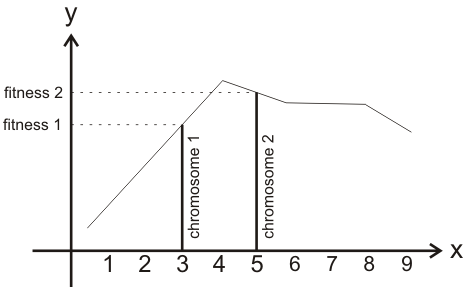
\includegraphics[width=0.8\textwidth]{images/1.png}
%\caption{}
\end{figure}
\end{frame}


\begin{frame}
\frametitle{Application Examples}
\begin{itemize}
\item Airlines Revenue Management
\item Automated computer designing
\item Bioinformatics
\item Code Breaking
\item Control engineering
\item Forensic science (facial composite construction)
\item Water distribution systems
\item Wireless sensor networks
\end{itemize}
\end{frame}


\begin{frame}
\frametitle{Genetic Algorithm Structure}
\begin{figure}
\centering
  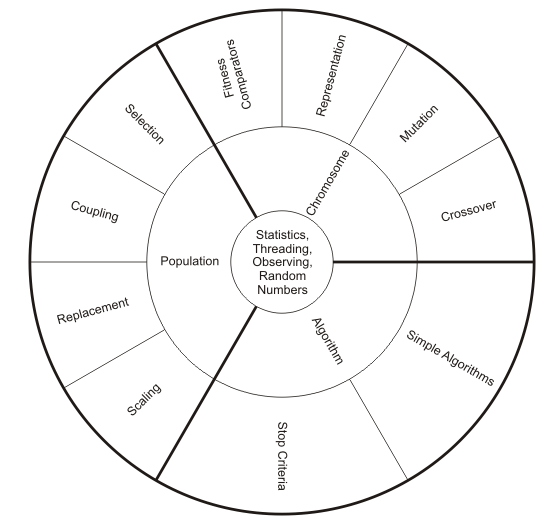
\includegraphics[width=0.6\textwidth]{images/2.png}
%\caption{Genetic Algorithm Structure}
\end{figure}
\end{frame}



\begin{frame}
\frametitle{Chromosomes}
-> Represented by the many solutions displayed by the genetic
algorithm which are labeled by fitness values. Through each generation
the algorithm selects the best chromosomes and combines them into
offsprings forming new populations until the best one is created and the
algorithm stops. They are composed by: \\
\bigskip
\begin{enumerate}
\item Fitness Comparators 
\item Representation
\item Mutation
\item Crossover
\end{enumerate}

\end{frame}


\section{Crossover}


\begin{frame}
\frametitle{Crossover Methods}
\begin{itemize}
\item Add Crossover
\item Midpoint Crossover
\item Multivalue Crossover
\end{itemize}
\end{frame}


\begin{frame}
\frametitle{Add/Sub Crossover}
The method implements the addition or subtraction of the entries of the two
individual’s chromosome, depending upon which of the methods was
invoked.
\end{frame}


\begin{frame}
\frametitle{}
\begin{figure}
\centering
  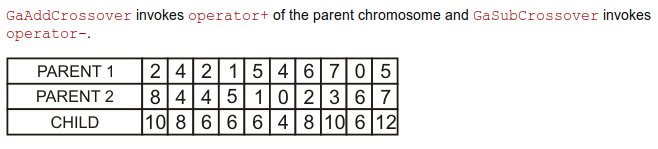
\includegraphics[width=0.8\textwidth]{images/3.png}
\caption{Sum}
\end{figure}
\begin{figure}
\centering
  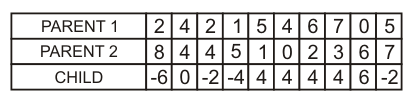
\includegraphics[width=0.5\textwidth]{images/4.png}
\caption{Subtract}
\end{figure}
\end{frame}



\begin{frame}
\frametitle{Midpoint Crossover}
This method implements a crossover operation which creates a child by invoking the Midpoint method of the chosen parents
\begin{figure}
\centering
  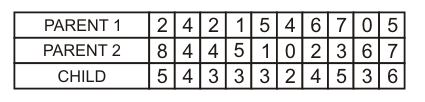
\includegraphics[width=0.8\textwidth]{images/5.png}
%\caption{Multivalue Crossover}
\end{figure}

\end{frame}



\begin{frame}
\frametitle{Multivalue Crossover}
The method implements a crossover operation which creates a child by choosing N cross points, and then it copies values from parents in turns, changing the source parent each time it reaches a chosen cross point.\\

\begin{figure}
\centering
  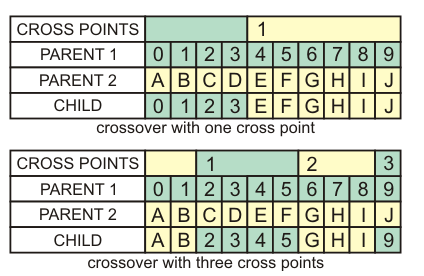
\includegraphics[width=0.6\textwidth]{images/6.png}
%\caption{Multivalue Crossover}
\end{figure}

\end{frame}





\section{Mutation}

\begin{frame}
\frametitle{Mutation Methods}
\begin{itemize}
\item Invert Mutation
\item Flip Mutation
\item Swap Mutation
\end{itemize}
\end{frame}




\begin{frame}
\frametitle{Flip Mutation}
Implements a mutation operation which chooses N values and sets them randomly.\\

\begin{figure}
\centering
  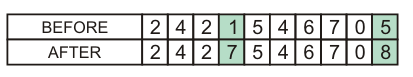
\includegraphics[width=0.6\textwidth]{images/8.png}
%\caption{Multivalue Crossover}
\end{figure}

\end{frame}


\begin{frame}
\frametitle{Invert Mutation}
The method implements a mutation operation which chooses N values and inverts them using the Invert method of the value set defined by the chromosome.\\

\begin{figure}
\centering
  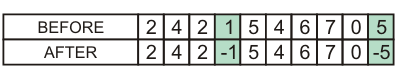
\includegraphics[width=0.6\textwidth]{images/7.png}
%\caption{Multivalue Crossover}
\end{figure}

\end{frame}



\begin{frame}
\frametitle{Swap Mutation}
Implements a mutation operation which chooses two blocks of values in a chromosome's code and swaps their positions in the code.\\

\begin{figure}
\centering
  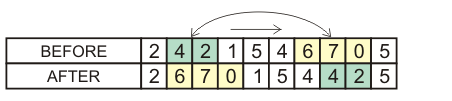
\includegraphics[width=0.6\textwidth]{images/9.png}
%\caption{Multivalue Crossover}
\end{figure}

\end{frame}




\begin{frame}[fragile]
\frametitle{C++ Implementation}
\lstset{language=C++}
\begin{lstlisting}
NOSE SI PONER ALGO O NO -_-
\end{lstlisting}
\end{frame}



\section{References}

\begin{frame}
\begin{enumerate} 
\item Janković, M. ., \textit{Genetic Algorithm Library}, April 7, 2012. \url{http://www.codeproject.com/Articles/26203/Genetic-Algorithm-Library}
\end{enumerate}
\end{frame}


\end{document}